% !TEX root = ../../main.tex

\section{Design Objectives}
\label{sec:design-objectives}

Our requirements are to provide a highly-available
and fast access to shared data, with uniform semantics across the
core-edge spectrum, while ensuring the strongest possible consistency
guarantees.

\system{} provides distributed access to shared data. A client
application process can execute transactions at an arbitrary node in
the cloud-edge spectrum, with uniform guarantees, enabling nodes or
code to migrate seamlessly.

In light of what we saw in the existing work, we will here justify
some protocol choices used in our approach, which aims to reduce shortcomings
observed in some existing systems.

We turn now to a system design for satisfying the above requirements
efficiently.
Our design is an extension of the SwiftCloud approach
\cite{rep:pan:sh177}.

\system{} uses caching and replication to ensure that a client can
execute locally.
The system must remain safe at all times; specifically, the data
observed by a client always satisfies the TCC+ and security invariants
defined below.
It should also remain available.

The trade-off is that, during some failures, liveness cannot be ensured.
A client cannot make progress in two cases: if it requires data that cannot be 
retrieved; or if it runs out of storage.
Furthermore, there are corner cases (described later) where a client
commits updates, but they cannot become visible.
The above situations are temporary, and last only until the problem is
repaired.

Our system ensures convergence by using operation-based CRDTs, which
merge concurrent conflicting operations deterministically \cite{syn:rep:sh143}.
As underlined in the Introduction, supporting causal consistency (CC)
can have high metadata overhead; our design bounds metadata to a small size.
Similarly to recent CC designs \cite{db:syn:1808, rep:pro:sh182},
\system{} separates (internal) state management from (external)
visibility: the backend layer transmits and stores states efficiently,
without regard for correctness, whereas the visibility layer manages
metadata and ensures that an application observes only those states that
satisfy the TCC+ guarantees.

\section{The TCC+ Guarantees}
\label{sec:tcc-guarantees}

We now tersely specify the TCC+ guarantees.
We use the following notations and definitions.
\begin{inparablank}
\item
  Nodes (at any level of the topology) are noted $p, p'$.
  A node behaves sequentially, executing one transaction at a time.
  A node might fail, in which case it ceases executing (fail-stop);
  a node that does not fail is said correct.
\item
  $x, y$ designate data objects.
\item
  Transactions are noted $T, T'$.
  A transaction consists of a sequence of reads and updates.
  A transaction is interactive, i.e., the objects it accesses are not
  known in advance.
  A read has no side effect; an update does not return a response value.
  We write $a \in T$ when operation $a$ (a read or an update) belongs to
  transaction $T$.
  A transaction executes at a single replica; if it commits, its updates
  are broadcasted to be replayed by the other replicas.
\item
  An operation is noted $a, b, \ldots{}$; in more detail, updating $x$
  is written $u(x)$, and a read $r(x)$.
  The response value of $r(x)$ is $\resp(r(x))$.
\end{inparablank}

Following \citet{rep:1754}, an abstract execution $A=(H,\vis,\ar)$
consists of
\begin{inparablank}
\item
  an interleaving of operations executed by the nodes, or history ($H$),
\item
  a visibility relation ($\vis$), a partial order that accounts
  for the propagation of updates in the system, and 
\item
  the arbitration relation ($\ar)$, a total order over $H$ that helps
  to resolve concurrency conflicts.
\end{inparablank}
%
The order in which nodes execute operations is called the program order.
The happened-before relation ($\hb$) is the transitive closure of the
union of visibility and program order \cite{rep:1754}.

Hereafter, we consider only transactions that commit; we can safely
ignore the operations of a transaction that aborts, since it has no
effect.

Note that, with TCC+, even a transaction that aborts reads a
consistent snapshot.


The phrase ``visible in node $p$'' refers to an operation
that is visible by some operation executed at node $p$.
%% FIXME never used.
%% The phrase ``$T$ at node $p$'' refers to a transaction
%% that first executes and commits at $p$, before being replicated to other nodes.

Each object starts in some known initial state.
The return value of a read is computed according to the semantics of
prior updates to the object (including updates in the same transaction).
That is, for each read operation $r(x)$, $\resp(r(x))$ results from some
linearization $l_{r(x)}$ of the updates visible to $r(x)$ consistent
with $\hb$.

TCC+ is defined by the following invariants.
\begin{inv}{Causal Consistency (CC)}
  Causal consistency requires that every update that happened-before an
  operation is visible to that operation, and that
  arbitration is consistent with happened-before.
  Formally, $(\happenedbefore \subseteq \vis) \land (\happenedbefore \subseteq \ar)$.
\end{inv}

\begin{inv}{Rollback-freedom}
  Once a node has read a value, it does not roll it back:
  If $r(x) \happenedbefore_{p} r'(x)$ then $l_{r(x)}$ prefixes $l_{r'(x)}$.
\end{inv}

\begin{inv}{Strong Convergence}
  Any two nodes that observe the same set of updates read the same value.
  Formally,
  $\forall r(x),r'(x):
  (\forall u(x); \visible{u(x)}{r(x)} \iff \visible{u(x)}{r'(x)})
  \implies \resp(r(x)) = \resp(r(x))$.
\end{inv}

The above invariants constrain the behavior of individual operations.
Below, we formalize the fact that a transaction is atomic (i.e.,
all-or-nothing).
%
We define the following equivalence relation, written $\equiv$: if
operations $a$ and $b$ are in the same transaction $T$, then $a \equiv b$.
%
For some relation $R$ over the set of operations, we say that $R$ is
left-compatible with $\equiv$ when for any three operations $a$, $b$ and
$c$, if $a \equiv b$ and $(a,c) \in R$ then $(b,c) \in R$.
Right-compatibility is defined symmetrically, that is $b \equiv c \land
(a,b) \in R \implies (a,c) \in R$.
Relation $R$ is compatible with $\equiv$ when it is both left- and
right-compatible with it.

\begin{inv}{Atomicity}
  If two updates occur in the same transaction, then they are visible
  atomically, and arbitrated in the same way.
  Formally, visibility and arbitration are compatible with transactional
  $\equiv$.
\end{inv}

\begin{inv}{Snapshot}
  A transaction takes all its reads (independently of their order) from
  a same snapshot, which is sound both causally and for the atomicity relation.
\end{inv}

Additionally, the following liveness property should hold:

\begin{inv}{Eventual Visibility}
  If two correct nodes $p$ and $p'$ are not permanently disconnected from one another,
  and $u(x)$ is visible in $p$, then eventually $u(x)$ is visible in $p'$.
\end{inv}

TCC+ extends Transactional Causal Consistency, as defined by
\citet{rep:pan:sh177}, with the Strong Convergence and Rollback-Freedom
properties.
This ensures that progress is monotonic at each node.

To illustrate the concepts in this section, consider the history in
Figure~\ref{fig:commit-protocol}, which depicts the evolution of a CRDT
counter ($x$) when nodes execute increment operations ($inc$), and
propagate such updates (depicted by arrows).%
%
\footnote{
  % 
  For now, ignore the version, commit and snapshot information, which will
  be detailed later.
}
%

The history in the figure is causally consistent.
Indeed, every new increment updates the counter to a state also
containing the preceding operations (e.g., after the event
\refevent{txn:TA2}, the counter value is $2$).
Similarly, there is no rollback at any node.
Nodes that received the same increments (e.g., events
\refevent{txn:TA1:DC0} and \refevent{txn:TA1:ack}) are in the same
state; therefore this history satisfies strong convergence.
Moreover, since every transaction contains a single operation, the
history trivially ensures the atomicity and snapshot requirements.

\section{Strengthening to SI}

\system{} strengthens the above TCC+ guarantees to strong consistency in an
SI zone.
Each DC forms a distinct SI zone.
Furthermore, a group of edge nodes in network proximity may elect to
form an SI zone (which an individual node can join or leave using
standard membership mechanisms).

In a SI zone, \system{} ensures Snapshot Isolation (SI).
This means that $\ar$ is gapless \cite{syn:formel:sh190}, i.e., for any
operation $b$ visible to $a$, every operation $c \ar b$ is also visible
to $a$.

\section{Bounding metadata}
\label{sec:bounding-metadata}

This and the following sections detail the logic to achieve the above
consistency guarantees.

Supporting CC requires metadata, which can represent a substantial
overhead; this section explains how \system{} bounds metadata to a small
size.

The CC invariant dictates that an update may become visible only
if its \emph{dependencies} (i.e., the updates that happened-before it)
are themselves visible.
To check this, when transmitting an update, \system{} piggy-backs some
associated \emph{visibility metadata}, a vector timestamp (or version
vector) that summarizes its dependencies \cite{alg:rep:738,
  alg:rep:738bis}.
Vector timestamps support efficiently computing the set
of missing dependencies \cite{rep:con:1414}.
(in contrast with storing explicit dependencies \cite{rep:syn:1662})

A precise representation of the happened-before order among $N$
concurrent writers requires a vector of size $\ge N$ \cite{syn:1707}.
As $N$ grows, the overhead on every message quickly becomes unacceptable.%
%
\footnote{
  % 
  In \system{} each component of the vector is 8 bytes, in order to
  store a monotonic clock that does not wrap around.
}
%
The following sections describe some techniques that we use
to keep the size small, at the cost of spuriously ordering some concurrent events.
\begin{inparaenum}[\textit (i)]
\item
  Since under SI writes are totally ordered, the set of nodes in an SI
  zone all count for one, and require only a single component.
\item
  The metadata for concurrent nodes connected to a common server node
  can be reduced to a scalar (called a \emph{dot}) on top of the vector
  \cite{rep:alg:1724}.
\item 
  As a safe approximation is sufficient to enforce the CC invariant,
  size $N$ can be made as small as desired \cite{rep:syn:1680}.
\item
  Connecting nodes in a tree of FIFO links also provides a safe
  approximation of CC, without added metadata \cite{db:syn:1808}.
\end{inparaenum}

\section{Topology and metadata design}
\label{sec:topology-metadata-design}

We first turn to the topology design (illustrated in
Figure~\ref{fig:topology}) and the metadata design.

Each DC forms an SI zone; therefore, the updates of a given DC are
totally ordered; externally, it behaves as a single sequential node.
On the other hand, DCs are connected in a full peer-to-peer mesh; their
updates are partially ordered, which requires a vector.
Since each DC appears sequential, a timestamp vector $V$ of size $N$
suffices to a point in the CC partial order between DCs.
Component $V[i]$ numbers the (sequentially ordered) transactions
committed at DC $i$.

The \emph{least upper bound} (LUB) of two vectors is defined as their
component-wise maximum.
Each node maintains its \emph{state vector}, which is the LUB of
the commit timestamps (defined next) that it has observed.

A transaction has a unique identifier called its \emph{dot}
\cite{rep:alg:1724}.

Successive transactions submitted at the same node have
monotonically-increasing dots.

Edge nodes (border or far-edge) are partitioned into distinct trees.
A tree is rooted at a specific DC, which we call its \emph{connected
  DC}\@.%
%
\footnote{
  % 
  A peer group counts for a single node in the tree.
}
%
This is illustrated in Figure~\ref{fig:topology}.
A subtree may detach itself from its parent and \emph{migrate} to a
different tree, e.g., to accommodate mobility or a failure.

\section{Transaction metadata}
\label{sec:transactions}

We now describe the metadata that \system{} associates with a
transaction $T$: its snapshot and commit timestamp vectors, and its dot.

Transaction $T$'s \emph{snapshot vector} $T.S$ describes the (previous)
transactions it depends upon.
$T.S$ forms a snapshot closed under causal consistency and atomicity.
The meaning of $T.S[j]=n$ is the following: $T$ reads from all the
transactions $T'$ committed at DC$j$ up to time $n$, and no later, i.e.,
such that $T'.C[j] \le n$.

A read-only or aborted transaction terminates without side effects.
The \emph{commit vector} $T.C$ of an update transaction represents the point
where it commits.%
% 
\footnote{
%
  In fact, to tolerate faults, it may have multiple equivalent commit
  vectors, as described later, in Section~\ref{sec:device-migration}.
}
%
It is greater than its snapshot vector; if the transaction commits at
DC$i$, they differ only at index $i$, i.e., $T.S[i] < T.C[i] \land
\forall j \neq i: T.S[j] = T.C[j]$, where $T.C[i]$ is a timestamp
assigned by DC$i$.

Transaction $T$ is before $T'$ if $T.C \le T'.S$.
If neither of $T$ or $T'$ is before the other, they are said concurrent.

Finally, a transaction has a unique timestamp called a \emph{dot} $T.D$,
which both serve as a unique identifier and provides the (total)
{arbitration order} between concurrent transactions
(as defined in Section~\ref{sec:tcc-guarantees}).

\begin{figure*}[tph]
  \centering
   % \includegraphics[scale=0.39]{fig/edge-commit-k-stability} %width=0.7\textwidth
  \hfill
  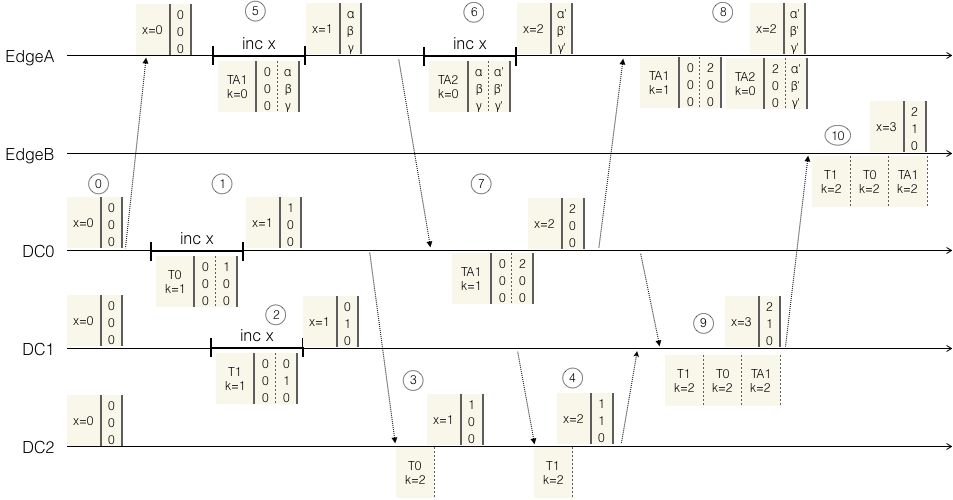
\includegraphics[scale=0.45]{figures/commit-protocol-main.png}
  \hfill
  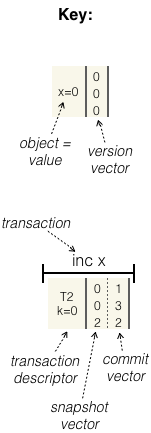
\includegraphics[scale=0.45]{figures/commit-protocol-key.png}
  \hfill
  % \vspace{-5mm}
  % \begin{quote}\footnotesize \noindent
  %   \labelevent{txn:init}{0}
\labelevent{txn:T0}{1}
\labelevent{txn:T1}{2}
\labelevent{txn:T0:DC2}{3}
\labelevent{txn:T1:DC2}{4}
\labelevent{txn:TA1}{5}
\labelevent{txn:TA2}{6}
\labelevent{txn:TA1:DC0}{7}
\labelevent{txn:TA1:ack}{8}
\labelevent{txn:T0TA1:DC1}{9}
\labelevent{txn:T0T1TA1:EdgeB}{10}


This system has three data centres DC0, 1, and 2, and edge nodes A and B.  Vector components refer to DC0, 1 and 2 respectively.  Dots are omitted from the figure.  The k-stability objective is 2.
\begin{description}[leftmargin=!,labelwidth=\widthof{\bfseries \refevent{txn:T0T1TA1:EdgeB}}]
\item[\refevent{txn:init}] Initially, the DCs observe $x=0$ with version vector $[0,0,0]$.
\item[\refevent{txn:T0}, \refevent{txn:T1}] Transaction T0 (resp.\ T1) increments $x$ at DC0 (resp.\ DC1), committing $x=1$ with version $[1,0,0]$ (resp.\ $[0,1,0]$).  Both have $k=1$.
\item[\refevent{txn:T0:DC2}] DC0 transmits T0 to DC2.  Being replicated at two DCs, it is 2-stable ($k=2$).
\item[\refevent{txn:T1:DC2}] DC1 transmits T1 to DC2.  T1 is now 2-stable. DC2 observes two increments, T0 and T1: now $x=2$ with version $[1,1,0]$, the least-upper-bound of the commit vectors of T0 and T1.
\item[\refevent{txn:TA1}] EdgeA caches $x$.  Transaction TA1 increments $x$ and commits locally.  Its commit vector remains the symbolic $[\alpha,\beta,\gamma]$.  As TA1 has not been transmitted to a DC, it has $k=0$.
\item[\refevent{txn:TA2}] Transaction TA2 at EdgeA again increments $x$.  Its snapshot vector is symbolic $[\alpha,\beta,\gamma]$; its commit vector is symbolic $[\alpha',\beta',\gamma']$.  The value of $x$ at EdgeA is now 2.
\item [\refevent{txn:TA1:DC0}] Concurrently, EdgeA transmits TA1 to DC0.  DC0 assigns commit vector $[\alpha,\beta,\gamma] := [2,0,0]$.  TA1 being known in one DC, it has $k=1$.  DC0 observes two increments, T0 and TA1: now $x=2$, with version $[2,0,0]$.
\item [\refevent{txn:TA1:ack}] DC0 transmits back the concrete descriptor of TA1, informing   EdgeA that $[\alpha,\beta,\gamma] = [2,0,0]$.  EdgeA observes local increments TA1 and TA2, hence $x=2$.  T0 is not visible to EdgeA because $T0.k=1$.
\item [\refevent{txn:T0TA1:DC1}] DC0 transmits T0 and TA1 to DC1, making them both 2-stable.
\item [\refevent{txn:T0T1TA1:EdgeB}] T0, T1 and TA1 being 2-stable at DC1, are made visible to EdgeB, where $x=3$.
\end{description}
Eventually (not depicted): TA2 is delivered to a DC, filling in the values for $[\alpha',\beta',\gamma']$; TA2 becomes 2-stable; all four transactions reach all replicas; all replicas observe $x=4$.

  % \end{quote}
  \caption{DC and edge transaction protocols}
  \label{fig:commit-protocol}
\end{figure*}

\paragraph{Figure~\ref{fig:commit-protocol} description:}
\labelevent{txn:init}{0}
\labelevent{txn:T0}{1}
\labelevent{txn:T1}{2}
\labelevent{txn:T0:DC2}{3}
\labelevent{txn:T1:DC2}{4}
\labelevent{txn:TA1}{5}
\labelevent{txn:TA2}{6}
\labelevent{txn:TA1:DC0}{7}
\labelevent{txn:TA1:ack}{8}
\labelevent{txn:T0TA1:DC1}{9}
\labelevent{txn:T0T1TA1:EdgeB}{10}


This system has three data centres DC0, 1, and 2, and edge nodes A and B.  Vector components refer to DC0, 1 and 2 respectively.  Dots are omitted from the figure.  The k-stability objective is 2.
\begin{description}[leftmargin=!,labelwidth=\widthof{\bfseries \refevent{txn:T0T1TA1:EdgeB}}]
\item[\refevent{txn:init}] Initially, the DCs observe $x=0$ with version vector $[0,0,0]$.
\item[\refevent{txn:T0}, \refevent{txn:T1}] Transaction T0 (resp.\ T1) increments $x$ at DC0 (resp.\ DC1), committing $x=1$ with version $[1,0,0]$ (resp.\ $[0,1,0]$).  Both have $k=1$.
\item[\refevent{txn:T0:DC2}] DC0 transmits T0 to DC2.  Being replicated at two DCs, it is 2-stable ($k=2$).
\item[\refevent{txn:T1:DC2}] DC1 transmits T1 to DC2.  T1 is now 2-stable. DC2 observes two increments, T0 and T1: now $x=2$ with version $[1,1,0]$, the least-upper-bound of the commit vectors of T0 and T1.
\item[\refevent{txn:TA1}] EdgeA caches $x$.  Transaction TA1 increments $x$ and commits locally.  Its commit vector remains the symbolic $[\alpha,\beta,\gamma]$.  As TA1 has not been transmitted to a DC, it has $k=0$.
\item[\refevent{txn:TA2}] Transaction TA2 at EdgeA again increments $x$.  Its snapshot vector is symbolic $[\alpha,\beta,\gamma]$; its commit vector is symbolic $[\alpha',\beta',\gamma']$.  The value of $x$ at EdgeA is now 2.
\item [\refevent{txn:TA1:DC0}] Concurrently, EdgeA transmits TA1 to DC0.  DC0 assigns commit vector $[\alpha,\beta,\gamma] := [2,0,0]$.  TA1 being known in one DC, it has $k=1$.  DC0 observes two increments, T0 and TA1: now $x=2$, with version $[2,0,0]$.
\item [\refevent{txn:TA1:ack}] DC0 transmits back the concrete descriptor of TA1, informing   EdgeA that $[\alpha,\beta,\gamma] = [2,0,0]$.  EdgeA observes local increments TA1 and TA2, hence $x=2$.  T0 is not visible to EdgeA because $T0.k=1$.
\item [\refevent{txn:T0TA1:DC1}] DC0 transmits T0 and TA1 to DC1, making them both 2-stable.
\item [\refevent{txn:T0T1TA1:EdgeB}] T0, T1 and TA1 being 2-stable at DC1, are made visible to EdgeB, where $x=3$.
\end{description}
Eventually (not depicted): TA2 is delivered to a DC, filling in the values for $[\alpha',\beta',\gamma']$; TA2 becomes 2-stable; all four transactions reach all replicas; all replicas observe $x=4$.


\section{In-DC transaction protocol}
\label{sec:dc-transaction-protocol}

Let us describe how the system computes metadata in the simple case
of a transaction that executes within some DC$i$.
By default, $T.S$ is assigned the current state vector of DC$i$.
The system checks that $T.S$ represents a consistent cut
\cite{rep:pro:sh182, rep:syn:sh156} such that $T.S[i] \le
\mathit{current\_time}$.
Its unique dot is $T.D := (\mathit{current\_time}, i)$.

When the transaction reads an object $x$, the system returns its
latest version included in the snapshot; choosing a snapshot vector
less or equal to the state of DC$i$ ensures that every read can be
satisfied. When the transaction updates $y$, the update is buffered,
and further reads of $y$ in the same transaction are satisfied from
the buffer.

The commit protocol is a standard two-phase commit among the
servers of DC$i$ (we use ClockSI \cite{rep:pan:1723}).
The commit vector is equal to the snapshot vector,
except that $T.C[i] := \mathit{current\_time}$.
Object versions created by the transaction are marked with version
timestamp $T.C$.

As \system{} objects are operation-based CRDTs, materializing a version
may require to apply multiple updates \cite{syn:rep:sh143,
  app:rep:1716}.
Conversely, concurrent transactions that update the same CRDT object can
be merged and by default do not abort, although it can abort for
semantic reasons, e.g., if it would violate some invariant; we assume a
higher level of concurrency control to detect such violations
\cite{syn:app:sh179, syn:rep:lan:1815, rep:syn:lan:1646}, which is out
of the scope of this paper.

When a DC receives a new remote transaction, it applies its updates to
the local store. Concurrent updates are merged according to CRDT
semantics; the merged version's timestamp is the least upper bound of
the corresponding commit timestamps.

We illustrate the in-DC transaction lifecycle in
Figure~\ref{fig:commit-protocol}, events \refevent{txn:init} through
\refevent{txn:T1:DC2}.
Focus on the three DCs, numbered 0, 1 and 2, and on the CRDT counter $x$.%
%
\footnote{
  % 
  Ignore for now the two edge nodes, and references to $k$ and
  to stability.
}
%
\begin{inparaenum}
\item[\refevent{txn:init}]
  All DCs have a copy of $x$ with value $0$ and version timestamp
  $[0,0,0]$.
  The three DCs are in state $[0,0,0]$.
\item[\refevent{txn:T0}]
  DC0 executes transaction T0.  Its snapshot vector is set from its
  current state, at $[0,0,0]$.
  T0 increments $x$.
  Its commit vector is $[1,0,0]$, i.e., its snapshot vector incremented
  by 1 at the component for DC0.
  It commits version $[1,0,0]$ of $x$, with value 1.
\item[\refevent{txn:T1}]
  Concurrently, DC1 executes T1, with the same snapshot.
  T1 also increments $x$.
  As $x$ is a CRDT, T1 can also commit; its commit vector is $[0,1,0]$
  and it updates $x$ to version $[0,1,0]$ with value 1.
  At this point, T0 is visible only to DC0, and T1 only to DC1.
\item[\refevent{txn:T0:DC2}]
  DC0 replicates T0 to DC2, where $x$ has version $[1,0,0]$.
\item[\refevent{txn:T1:DC2}]
  DC1 replicates T1 to DC2.
  All three versions of $x$ are visible at DC2, as well as a merged
  version with least-upper-bound timestamp $[1,1,0]$.
  As this version includes the increments from both T0 and T1, its value
  is 2.
\end{inparaenum}

\section{Basic Edge Transaction Protocol}
\label{sec:edge-trans-prot}

A transaction may execute and commit in an edge node.
In this case, commit is asynchronous, i.e., for
availability, the
edge node continues to execute further transactions without waiting for
the DC to assign its commit vector.

Starting a transaction $T$ is similar to the in-DC case: the edge node
assigns its snapshot, and a dot using the edge node's unique identifier.
The transaction commits locally at the edge node, which can immediately
start another dependent transaction.
Until it receives the DC's acknowledgement, the commit timestamp remains
\emph{symbolic}, i.e., indeterminate, subject only to the invariant $T.S
< T.C$.

Eventually, the edge node sends the transaction to its connected DC$i$,
which acknowledges with a concrete commit vector.
Similarly to the in-DC case, the commit vector differs from the snapshot
only in the component corresponding to the connected DC: $T.C[i] :=
\mathit{current\_time}$.
However, because of migration, index $i$ cannot be predicted, as
described in the next section.

Let us return to Figure~\ref{fig:commit-protocol} to illustrate
the lifecycle of edge transactions.
\begin{inparaenum}
\item [\refevent{txn:TA1}]
  Edge node A pulls $x$ into its interest set, then starts 
  transaction TA1 with snapshot vector $TA1.S = [0,0,0]$.
  TA1 reads version $[0,0,0]$ of $x$.
  TA1 increments $x$.
  TA1 commits; its commit vector is still uncertain, noted with the
  symbolic $TA1.C = [\alpha, \beta, \gamma] > [0,0,0]$.
\item [\refevent{txn:TA2}]
  EdgeA starts a second transaction TA2.
  To be able to read the writes of TA1 from the local cache, it assigns
  snapshot vector $TA2.S = [\alpha, \beta, \gamma]$.
  TA2 increments $x$ and commits with symbolic $TA2.C = [\alpha',
  \beta', \gamma'] > TA2.S = [\alpha, \beta, \gamma]$.
\item [\refevent{txn:TA1:DC0}]
  Concurrently, EdgeA sends TA1 to DC0.
  Similarly to an in-DC transaction, DC1 assigns the commit vector
  $TA1.C = [\alpha, \beta, \gamma] := [1,0,0]$.
\item [\refevent{txn:TA1:ack}]
  EdgeA receives the updated descriptor for TA1 and fills in the
  concrete values $TA1.C = TA2.S = [1,0,0]$.
\end{inparaenum}

\section{Node Migration and K-Stability}
\label{sec:device-migration}


The topology should be arranged to minimize response time and maximize
availability.
From this perspective, a fixed tree is inflexible, as a
single faulty link disconnects a whole subtree, and as latency changes
when a mobile node travels around.

A fixed tree is inflexible, and a single fault may have a
disproportionate impact.

Therefore, \system{} supports migrating a node and the subtree attached
to it.
Ideally, node migration should be seamless and  transparent to
applications, but unfortunately this is not completely possible.

Migration creates some extra complications to the edge transaction
protocol, which we consider next.
For simplicity, we focus on the case of a single migrating edge node.
Hereafter, we focus on the migration mechanism, and ignore the policy
decision of why or when to migrate, e.g., in response to a network failure.

\paragraph{Avoiding Duplicates}

Migration can change the connected DC of the node.
Consider the edge transaction protocol described above.
Suppose that some edge node sends its transaction $T$ to its connected
DC$i$, loses the connection to DC$i$, then migrates to DC$j \neq i$.
As the edge node does not know whether DC$i$ received $T$, it
sends $T$ again to DC$j$.
Although $T$ might now be received twice, via both DCs, a replica should
replay it only once; the transaction's dot $T.D$ serves to filter out
such duplicates.

According to causal ordering, dots must be received in monotonically
non-decreasing order.

To this effect, every node keeps track of the highest dot assigned by
another node, and ignores a transaction whose dot is less or equal this
value.

\paragraph{K-stability to avoid causal incompatibility}

The migrating edge node and its new connected DC$j$ each transmits the
updates it has visible and the other not.

Recall that snapshot $T.S$ was chosen less or equal to the state of
DC$i$, ensuring that its dependencies will be satisfied.

Consider an edge node that migrates from DC$i$ to a new connected DC$j$.
If the state of DC$j$ includes that of DC$i$, the edge node's
dependencies remain satisfied, and migration is seamless.
We say that the states are causally compatible.

However, it might happen (for instance, because of a communication
failure) that an edge transaction $T'$ depends on a transaction $T$ that was
visible at DC$i$ but not yet at DC$j$.
The snapshot of $T'$ does not satisfy the CC invariant at DC$j$, which
cannot apply it and cannot assign its commit vector.
The edge node remains effectively disconnected, and its 
transactions are non-visible to the rest of the system.
We say the edge node state is incompatible with DC$j$.

If $T$ was not visible to $T'$, the above dependency could not exist,
and the nodes would remain compatible.
Thus, one possible approach would be to let transaction $T$ become
visible at the edge only once it is known at all DCs.
However, a single slow DC would delay edge visibility of all 
transactions.

Our solution, taken from SwiftCloud \cite{rep:pan:sh177}, is twofold.
First, to ensure the Read-My-Writes session guarantee
\cite{rep:syn:1481}, an edge node's transactions are always visible to
itself.
Second, to decrease the probability of incompatibility, transaction
$T$ becomes visible to edge nodes only after it is visible by $\ge
K$ DCs, where $1 \le K \le N$ \cite{rep:pan:sh177}.
The higher $K$, the higher the probability that the new DC is compatible
with the old one, i.e., that its state includes the dependencies of
$T'$.
The exact value of $K$ is a trade-off between two extremes.
If $K=1$, the probability of incompatibility is high.
If $K=N$, a single slow DC could prevent all edge transactions from becoming
visible.  

To illustrate K-stability, refer again to
Figure~\ref{fig:commit-protocol}.
$T.k$ counts the number of DCs where $T$ is stable.
The visibility limit is set to $k \ge K = 2$.
At \refevent{txn:TA1:ack},

even though DC0 transmitted its state to EdgeA,

Transaction T0 is not visible to EdgeA, because $TO.k =
1$.
At \refevent{txn:T1:DC2}, DC1 sends T1 to DC2; now $T1.k=2$.
At \refevent{txn:T0TA1:DC1}, DC0 transmits T0 and TA1 to DC1; now all three transactions T0,
T1 and TA1 have $k=2$.
As DC1 has observed three increments, $x=3$ with version $[2,1,0]$, the
least-upper-bound $TC0.C, TC1.C$ and $TA1.C$.
Therefore, in \refevent{txn:T0T1TA1:EdgeB}, DC1 can make them visible to EdgeB, where later
transactions may depend on $x=3$ with version $[2,1,0]$.

\paragraph{Transaction Ordering}

Finally, both DC$i$ and DC$j$ may assign different commit vectors,
$T.C_{i} \neq T.C_{j}$.
This could cause an ordering anomaly: if some transaction $T'$ could
depend on $T$ with $T.C_{i} \le T'.S$, where $T.C_{j} \nleq T'.S$; a
node that knows only of $T.C_{j}$ is not aware that $T$ happens before
$T'$.
Observe, however, that $T.C_{i}$ and $ T.C_{j}$ conceptually denote the
same point in the TCC+ partial order.
To ensure this concretely, \system{} considers the two timestamps as
equivalent; they already have the same causal past, and the equivalence
ensures they have the same causal descendants.

Thus, a same transaction may carry up to $N$ equivalent commit
timestamps.

We optimize their memory size as follows.
Recall that a commit vector differs from the snapshot vector in a single
component, that of the DC that accepted it; the others
are not significant.
Therefore, \system{} stores multiple commit vectors into a single
vector of size $N$, containing a significant value only for a DC that
accepted the transaction.
For simplicity, Figure~\ref{fig:commit-protocol} does not depict
this optimization.

\section{Transaction Migration}
\label{sec:trans-migr}

Running at the edge provides fast response and high availability.
However, an edge device has limited resources, such as CPU capacity,
memory, power and bandwidth resources.
In contrast, the core cloud is rich in resources and can ensure better
consistency.
There is a trade-off and some computations are better placed in the
core.
Examples include analytics or large queries.
Although we expect edge execution to be the common case, \system{}
also supports moving a transaction from the edge, to execute in a
trusted environment at the connected DC\@.

If the state of the DC differs from the edge node, the result
might be inconsistent.
Thanks to TCC+, this is not an issue.
The result of a transaction depends only on its reads, i.e., on its
snapshot.
To ensure consistency, it suffices to run the transaction under the same
snapshot vector as if it was running on the client device.

Resource-hungry transactions should run in the core cloud rather than
the edge.
Examples include analytics or large queries.
\system{} supports migrating them to a trusted node in the core cloud
for execution.

The migrated transaction must have the same effect as if it ran on the
edge node; only performance should differ.
Thanks to TCC+, it suffices to assign the same snapshot vector.

Thus, the client primes the snapshot with its own state vector and sends
the transaction code.
Before the transaction starts, the DC must have received the client's
local transactions, which that the new one
depends upon (Section~\ref{sec:comm-outs-group} explains how we
accelerate this).

Since the edge node's state is less or equal the connected DC's, plus
its local transactions, this ensures that every read can be satisfied.

This ensures that every read can be satisfied.

The migrated transaction executes in the DC just like a standard local
client, and its results are sent back to the requesting edge node.
